\documentclass[12pt,a4paper]{article}
\pagestyle{plain}
\usepackage{fullpage}
\usepackage[english]{babel}
\usepackage{enumerate}

%equations
\usepackage[fleqn]{amsmath}
\numberwithin{equation}{section}

%figures
\usepackage[dvips]{graphicx}
\graphicspath{{./images/}}
\numberwithin{figure}{section}

%excercises
\newcounter{Exercise}
\setcounter{Exercise}{1}
\usepackage[dvipsnames]{xcolor}
\usepackage{framed}
\definecolor{shadecolor}{gray}{0.9}
\usepackage{caption}

%tables
\numberwithin{table}{section}

%specials
\usepackage{textcomp} %special (greek) characters as text
%\usepackage{pstricks} %
%\usepackage{ifthen} %
%\usepackage{calc} %
%\usepackage{isotope}
\usepackage{hyperref}
\usepackage[bottom]{footmisc} %footnote below figure
\usepackage{footnpag}%number footnotes per page
\usepackage{nicefrac}%fractions with slash


%document details
\author{N.G. Schultheiss \\ translated and adapted by K. Schadenberg}
\date{}
\title{Relativity}


\begin{document}
\maketitle

\section{Introduction}
In this module will try to explain what happens when two observers look at the same event. Every observer has his own coordinate system and clock (`frame of reference') with which the event is observed. These frames of references are not independent of each other. In this text we will deduce the relation between the two.

Some quantities are \textit{relative}, they depend on the observer, or more specifically the coordinate system of the observer. Other quantities are independent of the coordinate system, these are called \textit{invariant}. With this starting point we end up with Einstein's famous equation $E=mc^2$. In this text the entire derivation of this formula is written down. Study it carefully so you can make similar derivations on your own in the future.

\section{Lorentz and Poincar\'e}
Hendrik Antoon Lorentz is one of many Dutch Nobel prize laureates, he won the prize together with Pieter Zeeman. You might know Lorentz from the (equation for) Lorentz force $\textbf{F}_l = l(\textbf{I} \cdot \textbf{B})$. Lorentz won the Nobel prize for the discovery and theoretical explanation of the Zeeman effect.\footnote{The Zeeman effect describes the interaction between magnetic fields and the spin of particles. See module `Fluorescence' for more details.}

Lorentz was one of the first scientists to work on a theory of relativity (although it was not yet called relativity). To compare the observations of two observers we need to relate their frames of reference. This can be done with the use of the Galilean transformation:
\begin{equation}\label{eq:lorentz1}\begin{aligned}
x &= x' + vt' \\
y &= y' \\
z &= z' \\
t &= t'
\end{aligned}\end{equation}
Quantities without a prime mark are observed by the observer in the coordinate system without a prime mark. Quantities with a prime mark $'$ are observed by the second observer$'$ in the coordinate system$'$ with prime mark.\footnote{The prime mark is also used to denote the derivative of a function. When using the notation of equation \ref{eq:lorentz1} it is then unclear which derivative is meant, time or a specific space? To avoid confusion it is best to denote the derivative to a specific variable in the following manner: The derivative of the function $f(x,y,z,t)$ with respect to the time $t$ can be written as: $\frac{df(x,y,z,t)}{dt}$.}
In this example only the x-coordinate changes. This means that the second observer$'$ moved away from the first observer in the $x$ direction with a certain speed $v$.

Galileo Galilei assumed that time is the same in all frames of reference. However, when one approaches the speed of light this is no longer the case. The speed of light is a constant in the universe (invariant). Using the Galilean transformation we break this rule. We therefore need a different transformation method in which the speed of light remains constant. In this text we will only be looking at changes along the x-axis but all equations below can be expanded to also be valid for changes in other directions:
\begin{equation}\label{eq:lorentz2} \begin{aligned}
c &= \frac{\Delta x}{\Delta t} \\
c &= \frac{\Delta x'}{\Delta t'}
\end{aligned}\end{equation}

Lets look at a beam of light originating from the origin at $t=0$ travelling along the x-axis. We can use the following equations to calculate when this beam of light is observed at a certain position:
\begin{equation}\label{eq:lorentz3}\begin{aligned}
x &= ct \\
x' &= ct'
\end{aligned}\end{equation}
\begin{equation}\label{eq:lorentz4}\begin{aligned}
x - ct &= 0 \\
x' - ct'&= 0
\end{aligned}\end{equation}
The length of time can differ between the two frames, this allows us the write:
\begin{equation}\label{eq:lorentz5}
x' - ct' = \lambda (x - ct)
\end{equation}
For a beam of light travelling in the opposite direction:
\begin{equation}\label{eq:lorentz6}
x' + ct' = \mu (x + ct)
\end{equation}
Both equations are valid at the same time. Lets see if we can solve them.
\begin{itemize}
\item The sum of equations \ref{eq:lorentz5} and \ref{eq:lorentz6} yields:
\begin{align}\label{eq:lorentz789}
x' - ct' + x' + ct' &= \lambda (x - ct) + \mu (x + ct) \\
2x' &= (\lambda + \mu)x - (\lambda - \mu)ct \\
x' &= \frac{\lambda + \mu}{2}x - \frac{\lambda + \mu}{2} ct
\end{align}

\item The difference of equations \ref{eq:lorentz5} and \ref{eq:lorentz6} yields:
\begin{align}\label{eq:lorentz101112}
x' - ct' - (x' + ct') &= \lambda (x - ct) - \mu (x + ct) \\
-2ct' &= (\lambda - \mu)x - (\lambda + \mu)ct \\
ct' &= -\frac{\lambda - \mu}{2}x + \frac{\lambda + \mu}{2} ct
\end{align}
\end{itemize}

By introducing two new constants we can write the above equation in a more concise form:
\begin{align}\label{eq:lorentz1314}
a &= \frac{\lambda + \mu}{2} \\
b &= \frac{\lambda - \mu}{2}
\end{align}
\begin{align} \label{eq:lorentz15}
x' &= ax - bct \\ 
ct'&= -bx +act \label{eq:lorentz16}
\end{align}
Lets look at how fast the (coordinate) system$'$ is moving with respect to the system. We set $x'=0$:
\begin{align}\label{eq:lorentz171819}
0 &= ax - bct \\
v &= \frac{x}{t} = \frac{bc}{a} \\ 
\frac{v}{c} &= \frac{b}{a}\label{eq:lorentz19}
\end{align}
We can use this to expand equation \ref{eq:lorentz15}:
\begin{align}\label{eq:lorentz2021}
x' &= a\left( x -\frac{b}{a}ct\right)   \\
x' &= a\left( x -\frac{v}{c}ct\right) 
\end{align}
In a similar fashion we can rearrange equation \ref{eq:lorentz16}:
\begin{align}\label{eq:lorentz2223}
ct &= \frac{ct'}{a}+\frac{bx}{a}  \\
ct &= \frac{ct'}{a}+\frac{vx}{a}
\end{align}
Substitution yields:
\begin{align}\label{eq:lorentz24}
x' &= a\left( x-\frac{v}{c}\left( \frac{ct'}{a}+\frac{vx}{c}\right) \right) \\
x' &= a\left( 1-\left( \frac{v}{c}\right) ^2\right) x-a \frac{v}{c}\frac{ct'}{a}\\
x' &= a\left( 1-\left( \frac{v}{c}\right) ^2\right) x-vt' \label{eq:lorentz26}
\end{align}

We set our clocks in such a way that $t=t'=0$. For symmetry reasons a standard length which moves along with one coordinates system will always be observed in the same way from a second system$'$. From equation \ref{eq:lorentz15} follows:
\begin{equation}\label{eq:lorentz27}
x'=ax
\end{equation}
This means that a rod with a length of 1 (metre) in system$'$ will appear to have a length
\begin{equation}\label{eq:lorentz28}
x=\frac{1}{a}
\end{equation}
in system.

Because we set both times at zero, equation \ref{eq:lorentz26} becomes:
\begin{equation}\label{eq:lorentz29}
x' = a\left( 1-\left( \frac{v}{c}\right) ^2\right) x
\end{equation}
When one observes a rod of length 1 in system from system$'$, the rod will appear to have length:
\begin{equation}\label{eq:lorentz30}
x' = a\left( 1-\left( \frac{v}{c}\right) ^2\right)
\end{equation}
This transformation works both ways:
\begin{equation}\label{eq:lorentz31}
x=x'
\end{equation}
\begin{equation}\label{eq:lorentz32}
\frac{1}{a} = a\left( 1 \left( \frac{v}{c} \right)^2 \right) 
\end{equation}
\begin{equation}\label{eq:lorentz33}
a= \frac{1}{\sqrt{1-\left( \frac{v}{c} \right)^2}}
\end{equation}
Using equation \ref{eq:lorentz19}:
\begin{equation}\label{eq:lorentz34}
b= \frac{\frac{v}{c}}{\sqrt{1-\left( \frac{v}{c} \right)^2}}
\end{equation}
Substituting these formula in equations \ref{eq:lorentz15} and \ref{eq:lorentz16} yields:
\begin{align}\label{eq:lorentz3536}
x' &= \frac{x - vt}{\sqrt{1-\left( \frac{v}{c} \right)^2}} \\
t' &= \frac{t - \frac{v}{c^2}x}{\sqrt{1-\left( \frac{v}{c} \right)^2}}
\end{align}
This transformation, the Lorentz transformation, is different from the Galilean transformation. There is a new constant involved in the transformation, the Lorentz factor:
\begin{equation}\label{eq:lorentz37}
\gamma = \frac{1}{\sqrt{1-\left( \frac{v}{c} \right)^2}}
\end{equation}
\\ \indent Lorentz was a supporter of the `aether' theory and therefore had some trouble accepting his own equations. Jules Henri Poincar\'e had contact with Lorentz and together they improved the new theory of what would become Lorentz transformations and ultimately relativity. One of Poincar\'es suggestions was to imagine space as four dimensional (with time as one of the dimensions). The Lorentz transformations then describe this four dimensional world. If we define time as being imaginary in this space\footnote{Imaginary numbers are denoted by the symbol $i$, $i$ is defined as $i=\sqrt{-1}$.}, vectors always keep their length when transforming from one frame to another:
\begin{equation}\label{eq:lorentz38}
x^2+y^2+z^2-(ct)^2=x'^2+y'^2+z'^2-(ct')^2
\end{equation}

\section{Invariants}
In the previous sections we saw that quantities can change when we change our frame of reference. Not al quantities do so, those who do not are called invariant. Michelson and Morley showed with their experiment\footnote{See module `Michelson  Morley' for a description of the experiment and their results.} that the speed of light is invariant.

We can describe the state of an object using a position vector and time. Remember that most quantities are relative sush as these position vector and time. A more useful way of describing an object is by stating its momentum and energy. These two quantities can (and are) also used when describing collisions. Both momentum and location consist of three directions: $x$, $y$, and $z$. Time, according to Poincar\'e and Minkowski, is a fourth direction. When talking about momentum, energy can be seen as the fourth dimension.

The state of an object can thus be described as a four dimensional vector; 4-vector. The four components of a momentum/energy vector can be transformed from one system to another system$'$ which moves along it x-axis using the following equations:
\begin{equation}\label{eq:invar1}\begin{aligned}
p_x' &= \gamma \left( p_x - \beta \frac{E}{c} \right)  \\
p_y' &= p_y \\
p_z' &= p_z \\
\frac{E'}{c} &= \gamma \left( \frac{E}{c} - \beta p_x \right) 
\end{aligned}\end{equation}
In these equations $p$ denotes momentum and $E$ denotes energy. $\beta$ is a new variable, it describes how fast the systems are moving with respect to each other $\beta = \frac{v}{c}$ (compare this to the earlier variables $a$ and $b$). If we want to convert from the second system$'$ to the first $\beta$ will be negative. Using our new variable we can rewrite the Lorentz factor as $\gamma = \frac{1}{\sqrt{1-\beta^2}}$.

The length of the 4-vector can be determined using Pythagoras' theorem. If we take time or energy to be imaginary our 4-vector is invariant. Squaring the time or energy component will yield a negative number. Apparently the following equality holds:
\begin{equation}\label{eq:invar2}
p^2_{x'} + p^2_{y'} + p^2_{z'} - \left( \frac{E'}{c} \right)^2 = p^2_{x} + p^2_{y} + p^2_{z} - \left( \frac{E}{c} \right)^2
\end{equation}
We can verify if this is indeed true by substituting the equations from \ref{eq:invar1} into \ref{eq:invar2}:
\begin{equation}\label{eq:invar3}
\left( \gamma \left( p_x - \beta \frac{E}{c} \right)\right) ^2 + p^2_{y} + p^2_{z} - \left( \gamma \left( \frac{E}{c} - \beta p_x \right) \right)^2  = p^2_{x} + p^2_{y} + p^2_{z} - \left( \frac{E}{c} \right)^2 \Longrightarrow
\end{equation}
\begin{equation}\label{eq:invar4}
\left( \gamma \left( p_x - \beta \frac{E}{c} \right)\right) ^2 - \left( \gamma \left( \frac{E}{c} - \beta p_x \right) \right)^2  = p^2_{x} - \left( \frac{E}{c} \right)^2 \Longrightarrow
\end{equation}
\begin{equation}\label{eq:invar5}
\gamma^2 \left( p^2_x - 2p_x \beta^2 \left( \frac{E}{c}\right)^2\right)  - \gamma^2 \left( \left( \frac{E}{c}\right)^2 -2p_x\beta\frac{E}{c} +\beta^2 p^2_x\right) = p^2_x-\left( \frac{E}{c}\right)^2 \Longrightarrow
\end{equation}
\begin{equation}\label{eq:invar6}
\gamma^2 p^2_x -2\gamma^2 p_x \beta \frac{E}{c} + \gamma^2 \beta^2 \left( \frac{E}{c}\right)^2 - \gamma^2\left( \frac{E}{c} \right)^2 + 2\gamma^2 p_x \beta \frac{E}{c} - \gamma^2 \beta^2 p^2_x =p^2_x-\left( \frac{E}{c}\right)^2 \Longrightarrow
\end{equation}
\begin{equation}\label{eq:invar7}
\gamma^2 p^2_x - \gamma^2 \beta p^2_x - 2\gamma^2 p_x \beta \frac{E}{c} + 2\gamma^2 p_x \beta \frac{E}{c} + \gamma^2 \beta^2 \left( \frac{E}{c}\right)^2 - \gamma^2 \left( \frac{E}{c}\right)^2 =p^2_x-\left( \frac{E}{c}\right)^2 \Longrightarrow
\end{equation}
\begin{equation}\label{eq:invar8}
\gamma^2 \left( 1-\beta^2\right) p^2_x + \gamma^2\left( \beta^2 -1\right) \left(\frac{E}{c} \right)^2 =p^2_x-\left( \frac{E}{c}\right)^2 \Longrightarrow
\end{equation}
\begin{equation}\label{eq:invar9}
\frac{1-\beta^2}{1-\beta^2} p^2_x + \frac{\beta^2 -1}{1-\beta^2}\left(\frac{E}{c} \right)^2 =p^2_x-\left( \frac{E}{c}\right)^2 \Longrightarrow
\end{equation}
\begin{equation}\label{eq:invar10}
p^2_x-\left( \frac{E}{c}\right)^2 =p^2_x-\left( \frac{E}{c}\right)^2 
\end{equation}
Which proves that our 4-vector is invariant.

The length of this 4-vector can be related to another invariant; the (rest) mass. The next section will describe how Einstein deduced that when the momentum equals $p=\gamma mv$ the energy becomes $E=\gamma m c^2$. 
\begin{equation}\label{eq:invar11}
p^2-\left( \frac{E}{c}\right)^2 =(m \gamma v)^2 -\left(\frac{m \gamma c^2}{c} \right) = m^2 c^2 \gamma^2 \left( \left( \frac{v}{c}\right)^2 -1 \right) = 	m^2 c^2 \frac{\beta^2 -1 }{1-\beta^2}
\end{equation}
\begin{equation}\label{eq:invar12}
m^2 c^2 =\left( \frac{E}{c} \right)^2 - p^2
\end{equation}
Using this equation we can calculate the momentum of a photon. Recall that a photon does not have a (rest) mass and that therefore $p_{{photon}}=\frac{E_{{photon}}}{c}$, or according to Planck $p_{photon}=\frac{hv}{c}$.

If we choose our units in such a way that all quantities are expresses in terms of light speed and seconds\footnote{This is known as the Natural Units (NU) system. There are actually two NU systems; Lorentz-Heaviside and Gaussian. In both the speed of light is equal to 1 because they define $\varepsilon_0=1$ and $\mu_0=1$ ($c=\frac{1}{\varepsilon_0 \mu_0}$). Looking at the equations in this text is becomes clear why it is advantageous to set $c$ at 1, is greatly reduces the number of calculations.}, equation \ref{eq:invar12} can be written as:
\begin{equation}\label{eq:invar13}
m=\sqrt{E^2-p^2}
\end{equation}

Changing units is a method often used in physics and mathematics to make problems more clear. A different method is to make quantities dimensionless or `without units'. The variables $\beta$ and $\gamma$ in this text are examples of dimensionless quantities.

\section{Einstein and Minkowski}
Albert Einstein studied the recoil of light in a thought experiment and with this he came to his now famous equation $ E=mc^2$. He imagined a sealed box (in rest) with a certain length $l$ and mass $m_{box}$. On the left side of the box we send a photon to the right, after a certain time this photon will be absorbed by the right side of the box. We already mentioned how we can describe the momentum of a photon:
\begin{equation}\label{eq:einstein1}
p_{photon}=\frac{E_{photon}}{c}
\end{equation}
Furthermore:
\begin{equation}\label{eq:einstein2}
p_{box}=m_{box} v_{box}
\end{equation}
The speed of the box can be calculated by dividing the displacement of the box by the time the photon exists:
\begin{equation}\label{eq:einstein3}
p_{box}=m_{box} \frac{\Delta x_{box}}{\Delta t}
\end{equation}
Of course we must not forget the law of conservation of momentum. The box was stationary before the photon was emitted, therefore:
\begin{equation}\label{eq:einstein4}
m_{box} \frac{\Delta x_{box}}{\Delta t} + \frac{E_{photon}}{c} =0
\end{equation}
We know that photons travel at the speed of light, thus the box will move $\Delta t = \frac{l}{c}$ seconds.
\begin{equation}\label{eq:einstein5}
m_{box} \frac{\Delta x_{box}}{l} + \frac{E_{photon}}{c^2} =0
\end{equation}
If we know the displacement of the box we can solve this equality. We will now introduce a new quantity; $m_{photon}$. The law of conservation of momentum still holds\footnote{Here something strange happens, the photon will not traverse the entire length of the box if the box is moving in the opposite direction at the same moment. The assumption that the photon does travel the entire length only holds when the box has a far greater mass than the photon, can you explain why?. And on a side note; what happens with $\Delta t$?}:
\begin{equation}\label{eq:einstein6}
m_{photon} c + m_{box} v_{box} = 0
\end{equation}
\begin{equation}\label{eq:einstein7}
m_{photon} c \Delta t + m_{box} v_{box} \Delta t = 0
\end{equation}
\begin{equation}\label{eq:einstein8}
m_{photon} l + m_{box} \Delta x = 0
\end{equation}
Substitution in equation \ref{eq:einstein5} yields:
\begin{equation}\label{eq:einstein9}
m_{photon} = \frac{E_{photon}}{c^2}
\end{equation}
Generalising the equation above results in the famous equation:
\begin{equation}\label{eq:einstein10}
E=mc^2	
\end{equation}

Einstein's thought experiment tells us that when we put energy into an object, its mass will increase. In the previous section we saw that the length of the 4-vector is invariant. This means that the (rest) mass $m$ is also invariant. We now have two different masses, the rest mass and the apparent or observed mass. We will denote the observed mass as $M$:
\begin{equation}\label{eq:einstein11}
E=Mc^2=\alpha m c^2
\end{equation}
The observed mass $M$ is a factor $\alpha$ larger than the rest mass $m$\footnote{In most literature the rest mass is denoted as $m_0$, the observed mass is then written as $m$.}. Calculating the momentum is now done using:
\begin{equation}\label{eq:einstein12}
p=Mv=\alpha mv
\end{equation}
We can substitute this in equation \ref{eq:invar12}:
\begin{equation}\label{eq:einstein13}
m^2 c^2 =\left( \frac{\alpha m c^2}{c} \right)^2 - (\alpha m v)^2
\end{equation}
\begin{equation}\label{eq:einstein14}
m^2 = \alpha^2 m^2 \left(1-\left(  \frac{v}{c} \right)^2 \right)
\end{equation}
\begin{equation}\label{eq:einstein15}
\alpha^2 = \frac{1}{1-\left( \frac{v}{c} \right)^2 }
\end{equation}
\begin{equation}\label{eq:einstein16}
\alpha = \frac{1}{\sqrt{1-\left( \frac{v}{c} \right)^2}}
\end{equation}
Compare this $\alpha$ to the Lorentz factor $\gamma$, they are the same. The observed mass can thus also be written as $M=\gamma m$ and energy as:
\begin{equation}\label{eq:einstein17}
E=\gamma m c^2
\end{equation}

What this equation tells us is that an object, even when it is not moving, has a certain amount of energy. The classical equation for kinetic energy thus denotes a change in energy; $\Delta E=\frac{1}{2}mv^2$. In table \ref{tab:einstein1} and figure~\ref{einstein_vs_classical} the importance of this distinction at difference speeds can be seen. At low speeds both models give the same value (if we ignore the `mass energy' term). The classical model was constructed by Galilei, Huygens, Kepler, and Newton. They did not observe phenomena happening at the speed of light. So it is no surprise that their model could be in error at higher speeds. At $0.1~c$ the difference between the classical model and Einstein's model is less then 1\%. One tenth of the speed of light is 30000~km/s, compare this to the speed of weight falling from the Leaning Tower of Pisa in Galilei's experiments or the speed of the celestial bodies observed by Huygens and Kepler.
\begin{table}
\centering
\begin{tabular}{|r|r|r|}
\hline $\mathbf{v}$ & $\mathbf{E_{Einstein}}$ (J) & $\mathbf{\Delta E_{classical}}$ (J) \\ 
\hline 0c & $mc^2$ & 0 \\ 
\hline 0.1c & $mc^2$ + 0.005$mc^2$ & 0.005$mc^2$ \\ 
\hline 0.2c & $mc^2$ + 0.021$mc^2$ & 0.020$mc^2$ \\ 
\hline 0.3c & $mc^2$ + 0.048$mc^2$ & 0.045$mc^2$ \\ 
\hline 0.4c & $mc^2$ + 0.091$mc^2$ & 0.080$mc^2$ \\ 
\hline 0.5c & $mc^2$ + 0.155$mc^2$ & 0.125$mc^2$ \\ 
\hline 0.6c & $mc^2$ + 0.250$mc^2$ & 0.180$mc^2$ \\ 
\hline 0.7c & $mc^2$ + 0.400$mc^2$ & 0.245$mc^2$ \\ 
\hline 0.8c & $mc^2$ + 0.667$mc^2$ & 0.320$mc^2$ \\ 
\hline 0.9c & $mc^2$ + 1.294$mc^2$ & 0.405$mc^2$ \\ 
\hline 1.0c & $\infty$ & 0.500$mc^2$ \\ 
\hline 
\end{tabular}
\caption{Difference between the Einstein and classical model.}\label{tab:einstein1}
\end{table}

\begin{figure}\begin{center}
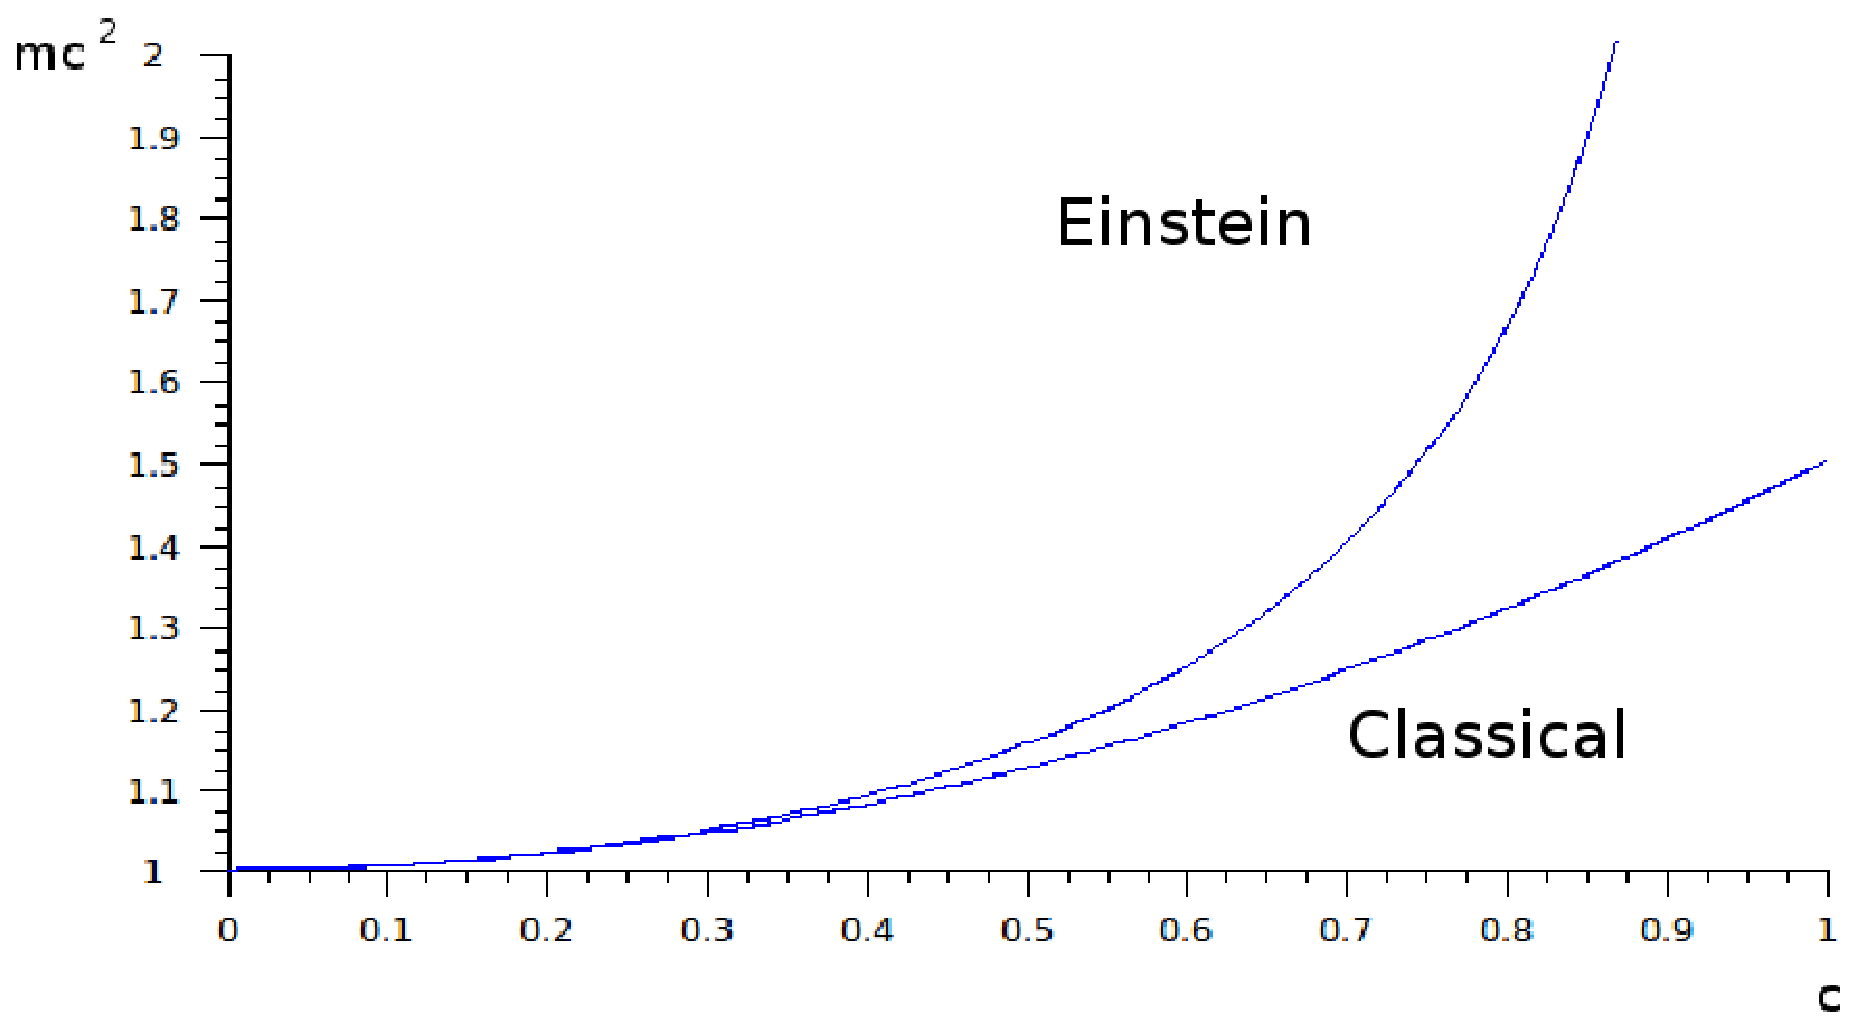
\includegraphics[scale=0.4]{einstein_vs_classical.eps}
\caption{The energy as function of the speed (in terms of c) according to Einstein and the classical model.}\label{fig:einstein_vs_classica}
\end{center}\end{figure}

At low speeds the classical model is a good approximation reality. However, at high speeds the error becomes unacceptably large. The speed of an object which has mass can never reach the speed of light. As you can see in table \ref{tab:einstein1} such an object would have an infinite amount of energy. Near the speed of light most of the energy you put into an object in `transformed' into mass. A direct consequence of this is that all particles travelling at the speed of light must have no rest mass.

With the laws for conservation of energy and momentum we should be able to do some calculations involving particles colliding at speeds near the speed of light.

While in Zurich, Albert Einstein was a student of Hermann Minkowski. During that time Minkowski was working at multidimensional mathematical problems. He took the ideas of Poincar\'e and expanded them into what we now call Minkowski space or Minkowski spacetime.

In 1915 Einstein expanded his special theory of relativity with the general theory of relativity. What was missing in the special theory was gravity. In the general theory gravity is explained as a curving of space(-time). Just at travelling at high speeds, gravity has an effect on time.

\paragraph{} \textbf{Exercise \theExercise \stepcounter{Exercise}} : In the sections `Invariants' and `Einstein and Minkowski' we run the risks of circle reasoning. Where does this risk occur and is this a problem?

\end{document}